\section{C Memory Model}

The C memory model is probably unlike most that you've seen before. Instead of allocating an object with type safety, we either use an automatic variable or request a sequence of bytes with \keyword{malloc} or another family member and later we \keyword{free} it.

\subsection{Structs}

In low-level terms, a struct is just a piece of contiguous memory, nothing more.
Just like an array, a struct has enough space to keep all of its members.
But unlike an array, it can store different types. Consider the contact struct declared above.

\begin{lstlisting}[language=C]
struct contact {
    char firstname[20];
    char lastname[20];
    unsigned int phone;
};

struct contact bhuvan;
\end{lstlisting}

We will often use the following typedef so we can just write contact contact1. One can also declare it in a single statement. 
\begin{lstlisting}[language=C]
typedef struct contact contact;
contact bhuvan;

typedef struct optional_name {
    ...
} contact;
\end{lstlisting}

If you compile the code without any optimizations and reordering, you can expect the addresses of each of the variables to look like this.

\begin{lstlisting}[language=C]
&bhuvan           // 0x100
&bhuvan.firstname // 0x100 = 0x100+0x00
&bhuvan.lastname  // 0x114 = 0x100+0x14
&bhuvan.phone     // 0x128 = 0x100+0x28
\end{lstlisting}

All your compiler does is say "reserve this much space, and I will calculate the offsets of whatever variables you want to write to'.
The offsets are where the variable starts at.
The phone variables starts at the \keyword{0x128}th bytes and continues for sizeof(int) bytes, but not always.
\textbf{Offsets don't determine where the variable ends though}. Consider the following hack that you see in a lot of kernel code.

\begin{lstlisting}[language=C]

typedef struct {
    int length;
    char c_str[0];
} string;

const char* to_convert = "bhuvan";
int length = strlen(to_convert);

// Let's convert to a c string
string* bhuvan_name;
bhuvan_name = malloc(sizeof(string) + length+1);
\end{lstlisting}

Currently, our memory looks like the following image.
There is nothing in those boxes

\begin{figure}[H]
\centering
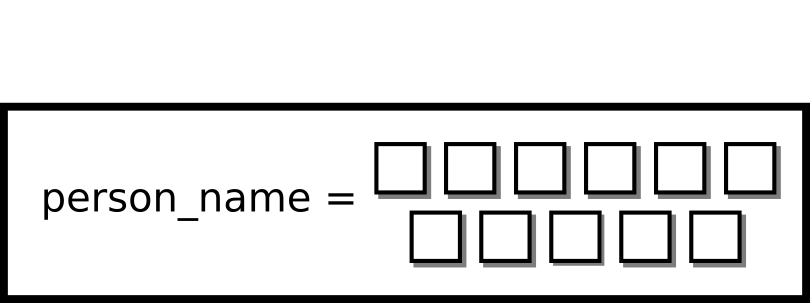
\includegraphics[width=.7\textwidth]{introc/drawings/memory_model_empty.png}
\caption{Struct pointing to 11 empty boxes}
\end{figure}

So what happens when we assign length?
The first four boxes are filled with the value of the variable at length.
The rest of the space is left untouched.
We will assume that our machine is big endian.
This means that the least significant byte is last.

\begin{lstlisting}[language=C]
bhuvan_name->length = length;
\end{lstlisting}

\begin{figure}[H]
\centering
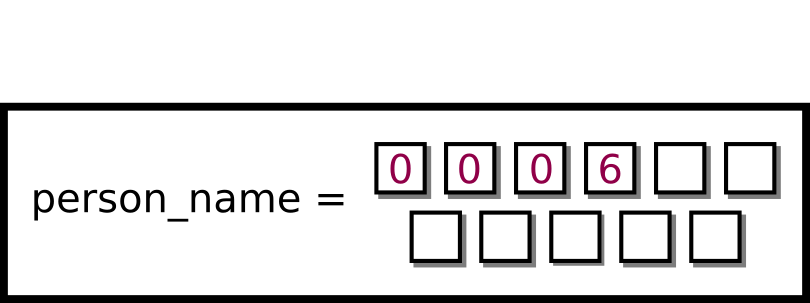
\includegraphics[width=.7\textwidth]{introc/drawings/memory_model_length.png}
\caption{Struct pointing to 11 boxes, 4 filled with 0006, 7 junk}
\end{figure}

Now, we can write a string to the end of our struct with the following call.

\begin{minted}{C}
strcpy(bhuvan_name->c_str, to_convert);
\end{minted}

\begin{figure}[H]
\centering
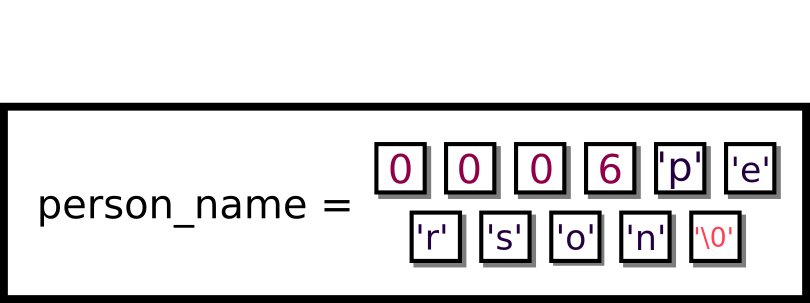
\includegraphics[width=.7\textwidth]{introc/drawings/memory_model_full.png}
\caption{Struct pointing to 11 boxes, 4 filled with 0006, 7 the stirng ``bhuvan''}
\end{figure}

We can even do a sanity check to make sure that the strings are equal.

\begin{minted}{C}
strcmp(bhuvan_name->c_str, "bhuvan") == 0 //The strings are equal!
\end{minted}

What that zero length array does is point to the \textbf{end of the struct} this means that the compiler will leave room for all of the elements calculated with respect to their size on the operating system (ints, chars, etc).
The zero length array will take up no bytes of space.
Since structs are just continuous pieces of memory, we can allocate \textbf{more} space than required and use the extra space as a place to store extra bytes.
Although this seems like a parlor trick, it is an important optimization because to have a variable length string any other way, one would need to have two different memory allocation calls.
This is highly inefficient for doing something as common in programming as is string manipulation.

\subsubsection{Extra: Struct packing}

Structs may require something called \href{http://www.catb.org/esr/structure-packing/}{padding} (tutorial).
\textbf{We do not expect you to pack structs in this course, just know that it is there} This is because in the early days (and even now) when you have to load an address from memory you have to do it in 32-bit or 64-bit blocks.
This also meant that you could only request addresses that were multiples of block sizes.
Meaning that

\begin{lstlisting}[language=C]
struct picture{
    int height;
    pixel** data;
    int width;
    char* encoding;
}
\end{lstlisting}

You think the picture looks like this.
One box is four bytes.

\begin{figure}[H]
\centering
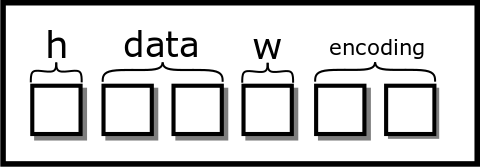
\includegraphics[width=.7\textwidth]{introc/drawings/struct_clean.png}
\caption{Six box struct}
\label{fig:clean_struct}
\end{figure}

However, with struct packing, it would conceptually look like this:

\begin{lstlisting}[language=C]
struct picture{
    int height;
    char slop1[4];
    pixel** data;
    int width;
    char slop2[4];
    char* encoding;
}
\end{lstlisting}

Visually, we'd add two extra boxes to our diagram

\begin{figure}[H]
\centering
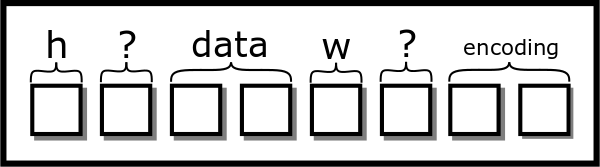
\includegraphics[width=.7\textwidth]{introc/drawings/struct_slop.png}
\caption{Eight box struct, two boxes of slop}
\label{fig:sloppy_struct}
\end{figure}

This padding is common on a 64-bit system.
This is not always the case because sometimes your processor supports unaligned access.
What does this mean?
We can have a variable start at a non-64-bit boundary.
The processor will figure out the rest.
To enable this, set an attribute.

\begin{lstlisting}[language=C]
struct __attribute__((packed, aligned(4))) picture{
    int height;
    pixel** data;
    int width;
    char* encoding;
}
\end{lstlisting}

Now our figure will look like the clean struct as in figure  \ref{fig:clean_struct}
But now, every time the processor needs to access \keyword{data} or \keyword{encoding},
two memory accesses are required.
The other thing you can do is reorder the struct, although this is not always possible

\begin{lstlisting}[language=C]
struct picture{
    int height;
    int width;
    pixel** data;
    char* encoding;
}
\end{lstlisting}

Which will get you the same output.

\subsection{Strings in C}

In C, we have
\href{https://en.wikipedia.org/wiki/Null-terminated_string}{Null
	Terminated} strings rather than
\href{https://en.wikipedia.org/wiki/String_(computer_science)\#Length-prefixed}{Length
	Prefixed} for historical reasons. What that means for your average everyday programming is that you need to remember the NUL character!
A string in C is defined as a bunch of bytes until you reach `\0' or the NUL Byte. `\0' is NULL casted to a character pointer.

\subsection{Places for strings}

Whenever you define a string literal - one in the form \keyword{char*\ str\ =\ "constant"} -- that string is stored in the \emph{data} section. Depending on your architecture, it is \textbf{read-only}, meaning that any attempt to modify the string will cause a SEGFAULT.
One can also declare strings to be either in the writable data segment or the stack. To do so, just specify a length for the string or put brackets instead of a pointer \keyword{char str[] = "mutable"} and put in the global scope or the function scope for the data segment or the stack respectively.
If one, however, \keyword{malloc}'s space, one can change that string to be whatever they want.
Forgetting to NUL terminate a string has a big effect on the strings! Bounds checking is important.
The heartbleed bug mentioned earlier in the book is partially because of this.

Strings in C are represented as characters in memory.
The end of the string includes a NUL (0) byte.
So "ABC" requires four(4) bytes.
The only way to find out the length of a C string is to keep reading memory until you find the NULL byte.
C characters are always exactly one byte each.

\subsubsection{String literals are constant}

A string literal is naturally constant.
Any write will cause the operating system to produce a SEGFAULT. 

\begin{lstlisting}[language=C]
char array[] = "Hi!"; // array contains a mutable copy
strcpy(array, "OK");

char *ptr = "Can't change me"; // ptr points to some immutable memory
strcpy(ptr, "Will not work");
\end{lstlisting}

String literals are character arrays stored in the code segment of the program, which is immutable.
Two string literals may share the same space in memory.
An example follows.

\begin{lstlisting}[language=C]
char *str1 = "Bhuvy likes books";
char *str2 = "Bhuvy likes books";
\end{lstlisting}

The strings pointed to by \keyword{str1} and \keyword{str2} may actually reside in the same location in memory.

Char arrays, however, contain the literal value which has been copied from the code segment into either the stack or static memory.
These following char arrays do not reside in the same place in memory.

\begin{lstlisting}[language=C]
char arr1[] = "Bhuvy also likes to write";
char arr2[] = "Bhuvy also likes to write";
\end{lstlisting}

Here are some common ways to initialize a string include. Where do they reside in memory?

\begin{lstlisting}[language=C]
char *str = "ABC";
char str[] = "ABC";
char str[]={'A','B','C','\0'};
\end{lstlisting}

\begin{lstlisting}[language=C]
char ary[] = "Hello";
char *ptr = "Hello";
\end{lstlisting}

We can also print out the pointer and the contents of a C-string very easily. Here is some boilerplate code to illustrate this.

\begin{lstlisting}[language=C]
char ary[] = "Hello";
char *ptr = "Hello";
// Print out address and contents
printf("%p : %s\n", ary, ary);
printf("%p : %s\n", ptr, ptr);
\end{lstlisting}

As mentioned before, the char array is mutable, so we can change its contents.
Be careful not to write bytes beyond the end of the array. C does \emph{not} do bounds checking at compile-time, but invalid reads/writes can get your program to crash.

Once again, be careful not to get the two mixed up!

\begin{lstlisting}[language=C]
strcpy(ary, "World"); // OK
strcpy(ptr, "World"); // NOT OK - Segmentation fault (crashes by default; unless SIGSEGV is blocked)
\end{lstlisting}

Unlike the array, however, we can change \keyword{ptr} to point to another piece of memory,

\begin{lstlisting}[language=C]
ptr = "World"; // OK!
ptr = ary; // OK!
ary = "World"; // NO won't compile
// ary is doomed to always refer to the original array.
printf("%p : %s\n", ptr, ptr);
strcpy(ptr, "World"); // OK because now ptr is pointing to mutable memory (the array)
\end{lstlisting}

Unlike pointers, that hold addresses to variables on the heap, or stack, char arrays (string literals) point to read-only memory located in the data section of the program. This means that pointers are more flexible than arrays, even though the name of an array is a pointer to its starting address.

In a more common case, pointers will point to heap memory in which case the memory referred to by the pointer \textbf{can} be modified.


